% Chapter Template

\chapter{System capabilities evaluation} % Main chapter title

\label{Chapter5} % Change X to a consecutive number; for referencing this chapter elsewhere, use \ref{ChapterX}

\lhead{Chapter 5. \emph{System capabilities evaluation}} 

In this chapter various capabilities of Indriya system have been evaluated. The evaluation has been done from a platform developer point of view. The features discussed ranges from intuitiveness to designing complex parallel behaviors on multiple robots. We describe how Indriya system could be used for realistic cases using example programs which would be otherwise extremely difficult to realize using existing methods for a novice programmer.
\section{Indriya: Sensible, intuitive and first of its kind}

In order to describe the simplicity and intuitiveness, we will make a comparative study of a scenario designed with Indriya and with that of Choregraphe behavior design software that comes with NAO humanoid robot. 
\begin{figure}[H]
\centering
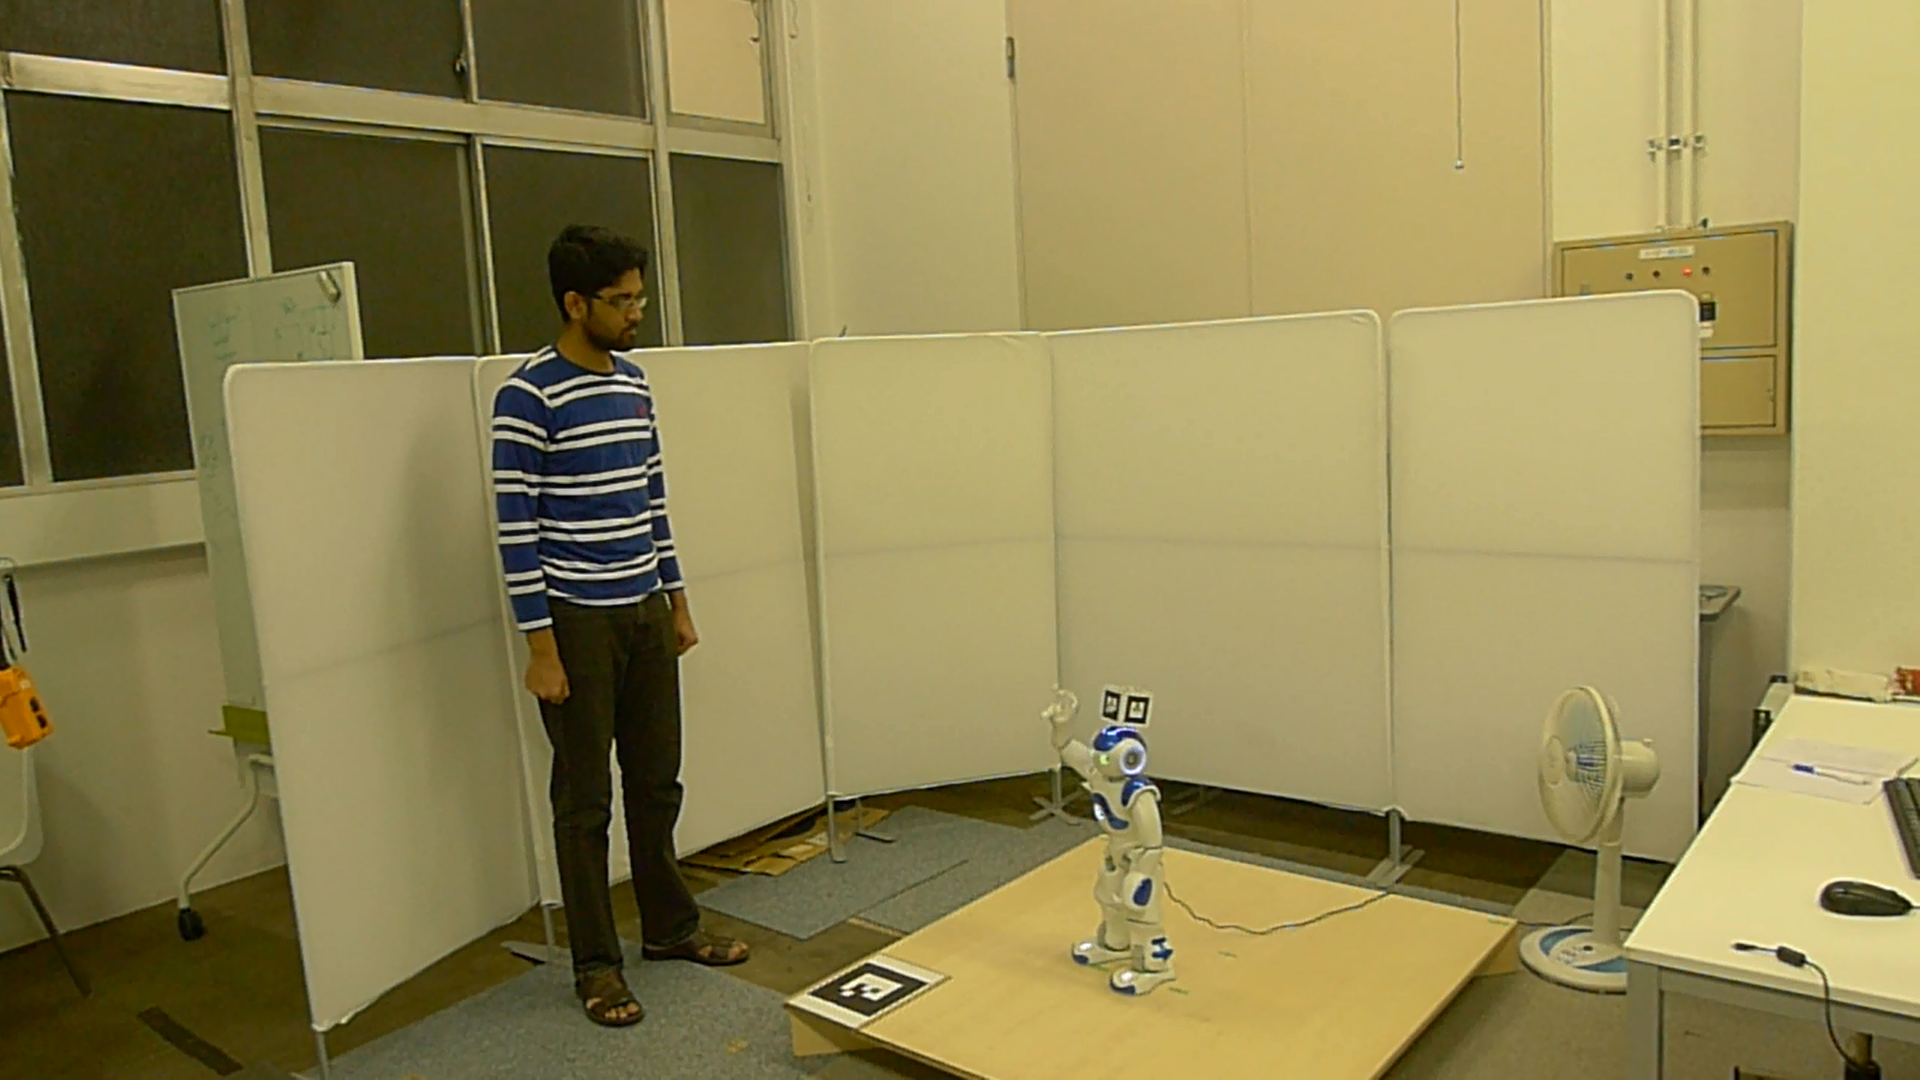
\includegraphics[width=0.8\textwidth]{../thesis/assets/scenario_museum.png}
\caption[NAO museum guide: Experiment setup]{NAO museum guide: Experiment setup}
\label{fig:scenario1_setup}
\end{figure}

\subparagraph{Scenario:}The NAO humanoid robot is a guide in a museum. The museum manager would like to design a scenario where when a visitor comes into the vicinity of the robot, the robot would approach him/her and start explaining the history of the museum. The experiment setup for this scenario is shown in Fig~\ref{fig:scenario1_setup}. We would like to use this scenario to compare the expressiveness and intuitiveness of behavior description with Choregraphe \cite{NaoRobot} shown in Fig~\ref{fig:scenario1_program_choregraphe} and with our interface shown in Fig~\ref{fig:scenario1_program}.

\begin{figure}[H]
\centering
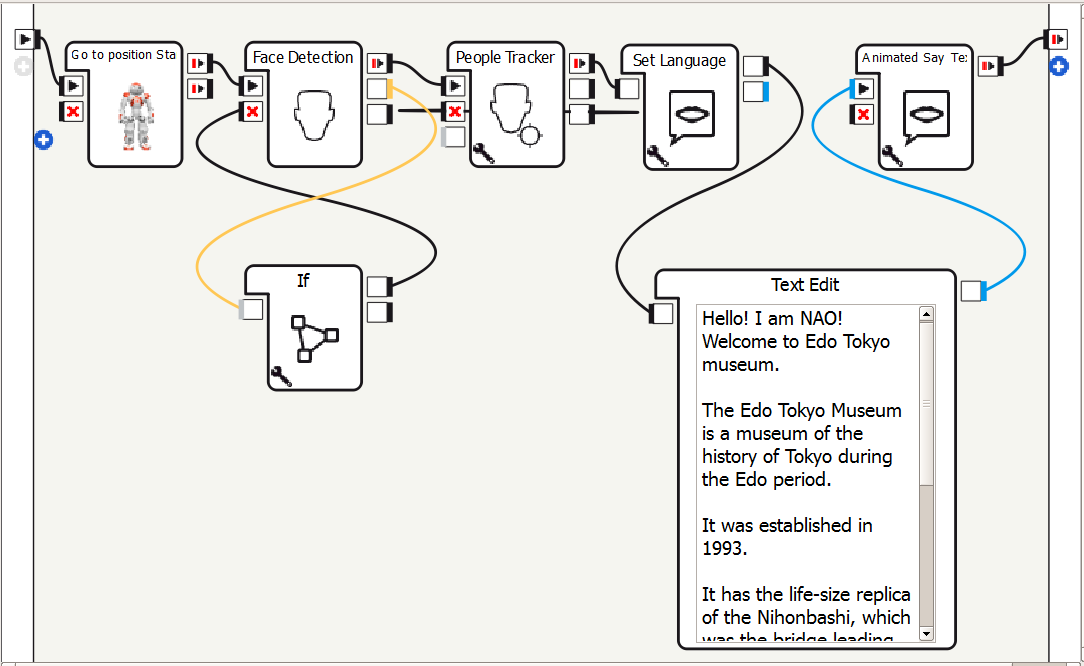
\includegraphics[width=\textwidth]{../thesis/assets/scenario_museum_choregraphe2.png}
\caption[NAO museum guide: Choregraphe Program]{NAO museum guide: Choregraphe Program}
\label{fig:scenario1_program_choregraphe}
\end{figure}

The behavior program desgined using Choregraphe software is shown in Figure~\ref{fig:scenario1_program_choregraphe}. Though Choregraphe uses a familiar flow-chart based programming model and has a huge library of primitive blocks to build complex motion patterns, the data flow for this scenario is not straight forward. As could be noticed from Fig~\ref{fig:scenario1_program_choregraphe}, at first the robot keeps looking for people in its vicinity using the \emph{Face detection block} at the cost of its power. The battery may be used up even before the robot really detects a person. Once it detects a person, the face detection block is stopped and \emph{People tracker} block is activated. The robot starts approaching (tracking) the person until a fixed distance with the person is reached. Once the desired distance of separation is achieved, the people tracker block has to be stopped. Now the robto will actually start explaining the history of the museum. It could be noticed that this kind of description/design of scenario might be easy for a seasoned programmer. However for a novice programmer it could be difficult to think of the dataflow as they literally have to emulate the whole scenario in their mind before designing the system. Moreover for human-in-the-loop scenarios like this, it is extremely difficult to simulate the behavior. So each time the behavior has to be executed in the real robot which increases the overhead of the design process.

Now let us see how such a scenario could be designed using Indriya system. The definition of this scenario is straightforward using Indirya as shown in Fig~\ref{fig:scenario1_program}.

\begin{figure}[H]
\centering
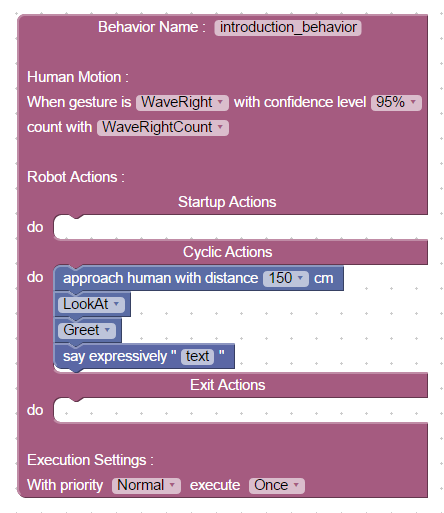
\includegraphics[width=\textwidth]{../thesis/assets/scenario1.png}
\caption[NAO museum guide: Indriya Program]{NAO museum guide: Indriya Program}
\label{fig:scenario1_program}
\end{figure}
		
The framework equipped with Kinect sensor takes care of the detection of people and gives the relative localization of the robot and human. Once the person is detected or a configured gesture trigger arrives, the behavior program retrieves the dynamic position of the robot and of the human from the application context. Using this information, the relative transformation of the human with respect to human is computed. The \emph{Approach block} makes use of this information to drive the robot towards the person. After coming into the proximity of the person, the robot starts explaining the history of museum configured using \emph{Say Expressively} block. From the user perspective, the design of the behavior is \emph{intuitive} using Indriya. He/She can focus on the scenario rather than thinking about the minute details of the data flow as the Indriya system equipped with the perception system acts as a proxy and eases the design process. 

\section{Realistic scenario design}
The Indriya system is not just for toy problems. In this section let us see how it could be used for realistic therapy scenario which is increasingly becoming important for rehabilitation. 
\subparagraph{Scenario:}A physiotherapist who is in a remote hospital would like to prepare an exercise routine for his patient who is recovering from the fracture of his left hand. The therapist wants the service robot in the rehabilitation center to give directions to the patient in an interactive manner and facilitate the process. The exercise is composed of: an introduction and demonstration of the routine, interactively reporting the progress of the exercise and finally notifying the completion. The experiment setup is shown in Figure~\ref{fig:scenario2_setup}
\begin{figure}[H]
\centering
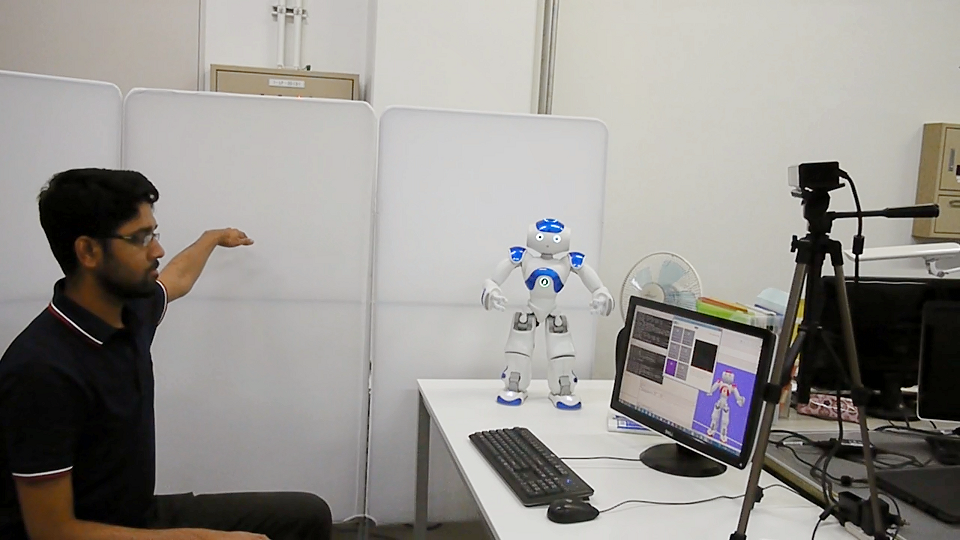
\includegraphics[width=\textwidth]{../thesis/assets/scenario_therapy.png}
\caption[NAO therapy facilitator: Experiment setup]{NAO therapy facilitator: Experiment setup}
\label{fig:scenario2_setup}
\end{figure}
Though Choregraphe software gives the capability of programming behaviors with basic human awareness, it does not explicitly allows programming that takes into account human gestures/motions. This is not the drawback of the system but the fact that it does not enough sensors to understand complex motions. Thanks to the Kinect sensor and its gesture recognition capabilites, we can exploit it design a program for the above scenario using Indriya system. A reference implementation of such a scenario using our behavior interface is shown in Fig~\ref{fig:scenario2_program}.
\begin{figure}[H]
\centering
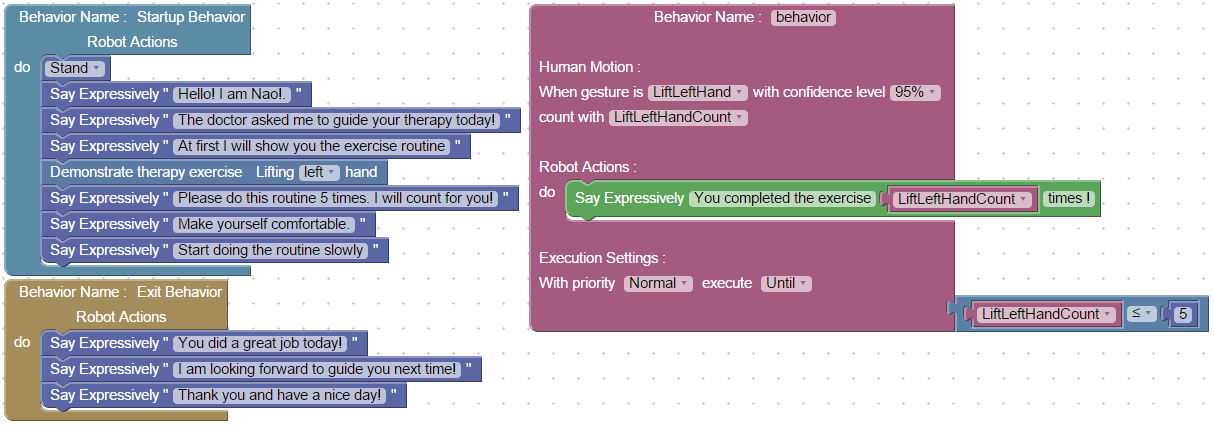
\includegraphics[width=\textwidth]{../thesis/assets/scenario2_horizontal.png}
\caption[NAO therapy facilitator: Indriya program]{NAO therapy facilitator: Indriya program}
\label{fig:scenario2_program}
\end{figure}
The above program is designed using all the three basic behavior constructs that constitutes the behavior program. In the Startup behavior the robot gives an introduction about the exercise routine and then gives a demonstration of how to do it. A trigger behavior block is configured to be triggered each time when the patient performs the therapy routine (lifting left hand). Inside the trigger behavior block in its startup block a variable is initialized to keep track of the count of the triggers. In the cyclic block, the variable is incremented and then the robot notifies the progress of the exercise by announcing how many times the patient has completed the exercise. The trigger behavior block is configured \emph{Until} a desired condition on the exercise count is reached (say lifting left hand 5 times). Once the lifetime of the trigger behavior block expires, the robot gives some closing comments about the routine. It could be noticed that the description of this scenario is quite simple using the Indriya. The blockly editor powered with the behavior program logic abstracts the complexity of designing realistic scenarios.
\section{Multi-robot programming at finger tips}
The Indriya system now supports NAO humanoid robot, Turtlebot and will soon support Pepper humanoid robot. The main advantage of the system is the robot interface modules developed for each of these robots are designed in such a way that it is easy to create multiple instances (nodes) dedicated for each robot with the same script by just changing the connection parameters as shown in Listing~\ref{lst:multirobot_config}

\lstinputlisting[caption=Sample XML Configuration File,label={lst:multirobot_config},language=XML]{assets/multirobot_config.xml}

In this way it is easy to extend the system to be used for many robots of same kind and also many different kinds of robots. The user interface is also designed in such a way that, it is easy to choose which action to be executed in which robot. The robot actions are categorized by their types in the tool box (Figure~\ref{fig:robot_categorize}) and with the given robot type it is possible to choose the robot by its name as specified by the user (Figure~\ref{fig:robot_selection}) in the configuration file. 

\begin{figure}[H]
\centering
\begin{subfigure}[t]{0.53\textwidth}
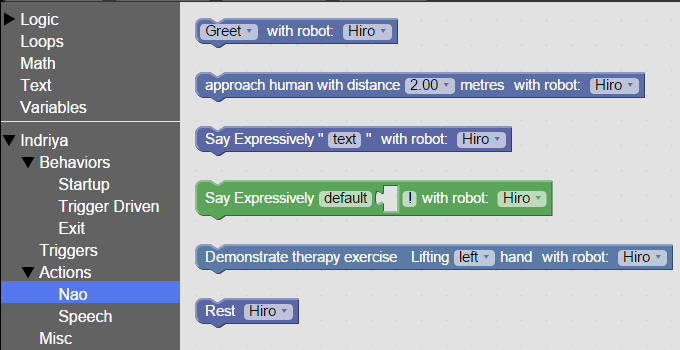
\includegraphics[width=\textwidth]{../thesis/assets/toolbox_multirobot.png}
\caption[Robot categorization]{Robot categorization}
\label{fig:robot_categorize}
\end{subfigure}
\hfill
\begin{subfigure}[t]{0.46\textwidth}
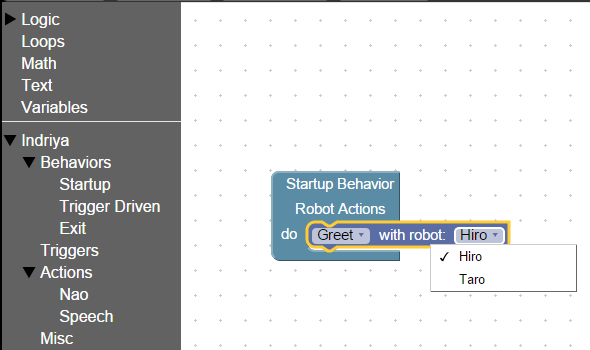
\includegraphics[width=\textwidth]{../thesis/assets/toolbox_multirobot2.png}
\caption[Individual robot selection]{Individual robot selection}
\label{fig:robot_selection}
\end{subfigure}
\caption[Multirobot support]{Multirobot support}
\label{fig:multirobot_support}
\end{figure}

\section{Parallel programming: Easier than ever before}
Collaborative introduction of Indriya system (2 Nao robots, 3 robots including turtlebot). 

\section{Priority execution making real sense}
Emergency stop scenario

\section{Summary and Discussion}

Speak about extensiblilty, modularity and software design